\documentclass[a4paper,12pt]{article}
\usepackage[utf8]{inputenc}
\usepackage{graphicx}
\usepackage{hyperref}
\usepackage{amsmath}
\usepackage{longtable}
\usepackage{tikz}
\usetikzlibrary{positioning, shapes.multipart, arrows.meta}
\usepackage[slovak]{babel}
\usepackage{url}


\usetikzlibrary{automata, positioning}

\renewcommand{\abstractname}{Abstrakt}
\renewcommand{\contentsname}{Obsah}
\renewcommand{\refname}{Referencie}
\renewcommand{\figurename}{Obrázok}
\renewcommand{\tablename}{Tabuľka}

\title{Dokumentácia vlastného protokolu nad UDP}
\author{Vladimír Jančár}
\date{\today}

\begin{document}

\maketitle

\begin{abstract}
   Táto dokumentácia má za úlohu podrobne opísať návrh a vysvetliť implementáciu komunikačnej aplikácie s využitím vlastného UDP protokolu. Najprv opisuje konkrétne časti hlavičky protokolu a ich úlohy. Ďalej dokument približuje konkrétne metódy, využívané na spoľahlivý prenos dát pomocou jednotlivých častí navrhovanej hlavičky. Na záver rozpráva o implementácii tohto protokolu pomocou vlastnej komunikačnej aplikácie.
\end{abstract}

\tableofcontents

\section{Úvod}
	Tento protokol je určený na peer-to-peer komunikáciu v lokálnej Ethernet sieti a umožňuje prenos textu alebo súborov systémom Stop-and-Wait Automatic Repeat Request. Na nadviazanie spojenia využíva 3-Way Handshake, pričom stabilitu spojenia zabezbečuje keep-alive systém. Vďaka kontrolnému súčtu CRC16 a poradovým číslam packetov protokol chráni integritu prenášaných údajov a s fragmentáciou umožňuje aj posielanie väčších súborov. Hlavnou výhodou tohto protokolu je jednoduchosť, pričom nezanedbáva kľúčové vlastnosti ako detekciu chýb, spoľahlivé doručovanie správ alebo udržiavanie spojenia.

\section{Návrh protokolu}

    Protokol je navrhutý nad UDP, no jeho cieľom je zaručovať spoľahlivý prenos dát, a preto napodobňuje funkčnosť TCP. Zabezpečuje nadviazanie spojenia medzi dvoma stranami podobne ako TCP 3-way handshake. Zvláda prenášať väšie súbory vďaka fragmentácii dát. V prípade, že overenie integrity zlyhá, poškodené dáta sa pošlú znova. Protokol umožňuje aj udržanie aktívneho spojenia medzi uzlami vďaka pravidelnej kontroly druhej strany spojenia.


    \subsection{Hlavička protokolu}

  
    Hlavička vlastného protokolu je veľkosti 88 bitov a je štruktúrovaná nasledovne:
    \begin{longtable}{|l|l|l|}
        \hline
        \textbf{Pole} & \textbf{Veľkosť} & \textbf{Popis} \\
        \hline
       % Source port & 16b & Port odosielajúceho uzla \\
        %Destination port & 16b & Port prijímajúceho uzla \\
	Acknowledgement number & 16b & Poradové číslo prijatého paketu \\
        Sequence number & 16b & Poradie paketu \\
        Fragment & 8b & Poradie fragmentu \\
        Total fragments & 8b & Celkový počet fragmentov \\
        ACK & 1b & Acknowledgement flag \\
        SYN & 1b & Synchronization flag \\
        FIN & 1b & Finish flag \\
        ERR & 1b & Error flag \\
        Reserved & 4b & Nevyužité bity \\
        Checksum & 16b & Kontrolná hodnota CRC16 \\
        Data length & 16b & Dĺžka prenášaných údajov \\
        \hline
    \end{longtable}

	Diagramová reprezentácia štruktúry hlavičny je vyjadrená v obrázku~\ref{fig:header}.

   \begin{figure}[h]
        \centering
        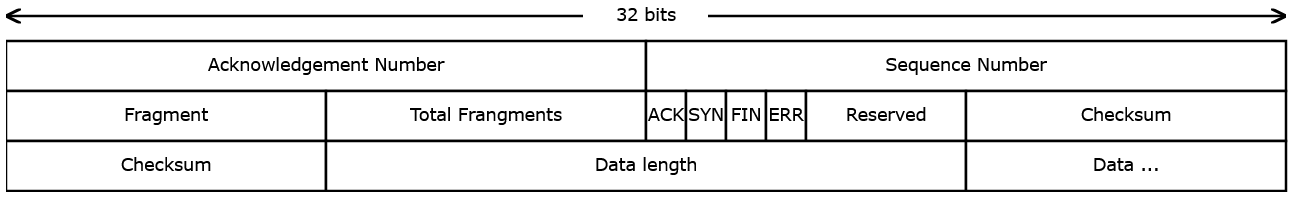
\includegraphics[width=1\textwidth]{protocol_1.png}
        \caption{Štruktúra hlavičky protokolu}
        \label{fig:header}
    \end{figure}

    \subsection{Popis polí}
    \begin{itemize}
        %\item \textbf{Zdrojový port}: Port používaný odosielateľom. Umožnuje prijímateľovi posielať odpovede.
        %\item \textbf{Cieľový port}: Port používaný prijímateľom. 
	\item \textbf{Acknowledgement number}: Pri potvrdení správnosti packetu toto pole obsahuje poradové číslo prijatého packetu.
        \item \textbf{Číslo sekvencie}: Pomáha kontrolovať správne poradie poslaných správ alebo súborov, čo je užitočné najmä pri fragmentácii.
        \item \textbf{Číslo fragmentu a celkový počet fragmentov}: Prijímateľ tieto údaje potrebuje na správne poskladanie prijatých fragmentov, prípadne na zistenie, či niektoré fragmenty nechýbajú.
        \item \textbf{ACK, SYN, FIN, ERR}: Riadiace flagy slúžiace na nadviazanie spojenia pomocou 3-way handshake, ukončenie spojenia a indikáciu chybných packetov.
        \item \textbf{Checksum}: Kontrolná hodnota pre zistenie poškodenia prenášaných údajov.
        \item \textbf{Dĺžka údajov}: Očakávaná dĺžka prenášaných údajov v bytoch.
    \end{itemize}

    \subsection{Kontroly integrity}\label{crc}
    K zabezpečeniu integrity prenášaných údajov využíva protokol 16-bitovú cyklickú kontrolu (CRC16) na výpočet kontrolného súčtu - \textbf{checksum}. Odosielateľ pred poslaním správy vypočíta jej checksum a vloží ho do hlavičky protokolu. Prijímateľ po prijatí správy vypočíta jej checksum znova a porovná ho s číslom v hlavičke protokolu. Ak sa zhodujú, správa nebola počas prenosu poškodená a prenos dát pokračuje. V prípade nezhody je odosielateľovi poslaná odpoveď s chybovým flagom ERR a poškodené dáta sa pošlú znova. Postup pri zaznamenaní poškodenia je podrobnejšie opísaný v časti \ref{prenos}.

Kontrolný súčet je 16-bitová hodnota vypočítaná nasledovne:
	\begin{enumerate}
		\item Najprv si vyberieme mnohočlen, ktorý budeme používať pri výpočte hodnoty CRC. Pre CRC16 sa bežne používa:
		\[ P(x) = x^{16} + x^{15} + x^2 + 1 \] (V hexadecimálnom tvare \textbf{0x8005})
		
		\item Nastavíme počiatočnú CRC hodnotu. Zvyčajne sa používa \textbf{0xFFFF}.
		
		\item Postupne prechádzame vstupnými dátami. Každý byte údajov ktoré kódujeme, prejde nasledujúcimi krokmi:
		\begin{enumerate}
		    \item XOR-ujeme byte s najvššími ôsmimi bitmi hodnoty CRC.
		    \item Pozrieme sa, či má najvyšší bit hodnotu 1. Ak áno, spravíme bitový posun hodnoty CRC doľava a XOR-ujeme ju s vybraným mnohočlenom. Ak nie, spravíme iba bitový posun CRC doľava. 
		    \item Ak sme ešte neprešli všetky bity v byte, vrátime sa do kroku (a).
		\end{enumerate}

		\item Nazáver XOR-ujeme CRC hodnotu s 0xFFFF, ako je štandardom pri CRC-16-IBM, ktorý sme sa snažili napodobniť.
    \end{enumerate}

    \subsection{Spoľahlivý prenos údajov}\label{prenos}
    Protokol zabezpečuje spoľahlivý prenos údajov spôsobom \textbf{Stop \& wait Automatic Repeat Request (S\&W ARQ)}. To znamená, že po každom poslanom packete musí odosielateľ čakať na odpoveď od prijímateľa. Na základe tejto odpovede sa buď pošle packet znova, alebo sa pošle ďalší. Celý proces vyzerá nasledovne:

    \begin{enumerate}
        \item Odosielateľ pošle packet so špecifickým poradovým číslom (sequence number)\footnote{ide o globálne poradie, takže každá správa má vlastné číslo. V prípade, že sa dovŕši maximum, poradie začína opäť od nuly. Pri fragmentácii (\ref{frag}) majú všetky fragmenty rovnaké poradové číslo.} a čaká na odpoveď od prijímateľa. 
	\item Na základe odpovede môžu nastať tieto prípady:	
	\begin{itemize}        
		\item Ak nedostane odosielateľ odpoveď do 250ms, vyšle rovnaký packet znova a čaká. To sa opakuje až kým nedostane odpoveď alebo kým nie je komunikácia prerušená.
		\item Keď je v prijatom packete nájdená chyba (checksum od odosielateľa sa nezhoduje s checksumom vypočítaným prijímateľom), odošle sa ako odpoveď packet s rovnakým poradovým číslom v Acknowledgement field a ERR flagom s hodnotou 1. Odosielateľ po tejto odpovedi pošle rovnaký packet znova.
	        \item Ak je prijatý packet v poriadku, odošle sa odpoveď vo forme packetu s rovnakým poradovým číslom v acknowledgement field a ACK flagom s hodnotou 1.
   	\end{itemize}
    \end{enumerate}

    \subsection{Nadviazanie spojenia}
	Predtým, než bude možné si vymienať údaje, musia sa oba uzly presvedčiť, že druhá strana je pripravená komunikovať. K tomuto účelu slúži tzv. \textbf{3-Way Handshake} (Obr. \ref{fig:handshake_diagram}), ktorý pozostáva z nasledujúcich krokov:
	
	\begin{enumerate}
	    \item 
		Odosielateľ žiadosti o nadviazanie spojenia pošle packet s vlajkou \textbf{SYN=1} a poradovým číslom X \textbf{(Seq=X)}.
	    \item 
		Keď prijímateľ dostane SYN packet, odošle odpoveď: tzv. SYN-ACK packet s vlajkami \textbf{SYN=1} a \textbf{ACK=1}. Packet bude obsahovať polia \textbf{(Seq=Y)} a \textbf{(Ack=X+1)}.
	    \item 
		Nakonie iniciátor spojenia na SYN-ACK packet odpovie odoslaním ACK packetu, kde \textbf{(Ack=Y+1)}. Potom je spojenie úspešne naviazané.
	\end{enumerate}

	\begin{figure}[h]
		\centering
		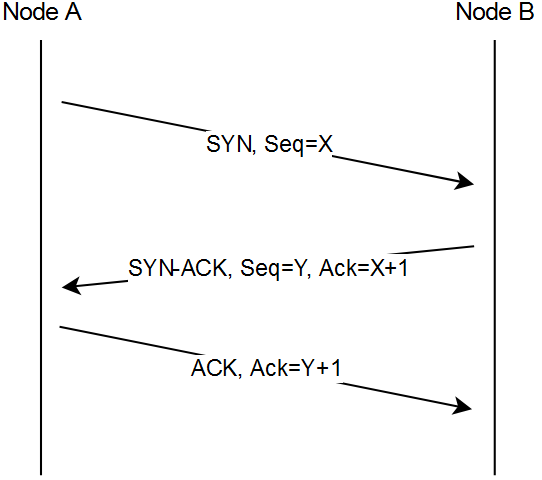
\includegraphics[width=0.70\textwidth]{handshake_diagram.png}
		\caption{Diagram procesu nadviazania spojenia}
		\label{fig:handshake_diagram}
	\end{figure}
	

    \subsection{Udržanie spojenia}\label{keepalive}
	Pre udržanie spojenia medzi dvoma uzlami využíva protokol metódu \textbf{Keep-Alive}. Aby sa predišlo strate spojenia v prípade, že ani jedna strana neposiela údaje, vymieňajú si uzly tzv. \textbf{heartbeat packety} každých 5 sekúnd nečinnosti. Takýmto spôsobom protokol zisťuje, či sú obe strany stále pripojené. Heartbeat packety vyzerajú tak, že ich ACK flag má hodnotu 1 a ich poradové číslo je 0. Ak jedna zo strán nedostane odpoveď na 3 po sebe odoslané heartbeat packety, spojenie sa považuje za ukončené. Vtedy nastane jedna z nasledujúcich situácií:

	\begin{itemize}
	\item Ak nedostane komunikátor odpoveď na žiaden z heartbeat packetov, vypíše informačnú správu pre používateľa o ukončení spojenia. V prípade, že sa spojenie prerušilo počas prenosu textu alebo súboru, vypíše aj to, že prenos zlyhal.
	\item Ak sa podarí obnoviť spojenie (komunikátor dostane odpoveď aspoň na posledný odoslaný heartbeat packet) a prerušenie nastalo počas prenosu textu alebo súboru, pokúsi sa v pokračovať v prenose tam, kde sa spojenie prerušilo.
   	\end{itemize}

	\subsection{Ukončenie spojenia}
		V protokole prebieha ukončenie spojenia podobne ako pri TCP (4-way termination) (Obr \ref{fig:disconnect_diagram}). Proces vyzerá nasledovne:
		\begin{enumerate}
			\item Odosielateľ pošle packet s flagom \textbf{FIN=1} a poradovým číslom (Seq=X).
			\item Po prijatí FIN packetu druhý uzol odpovie odoslaním packetu s flagom \textbf{ACK=1} a rovnakým poradovým číslom. Následne odošle aj FIN packet s novým poardovým číslom (Seq=X+1).
			\item Prvý odosielateľ po prijatí FIN packetu odošle posledný ACK packet, čím definitívne potvrdzuje ukončenie spojenia.

		\end{enumerate}
			
		\begin{figure}[h]
		    \centering
		    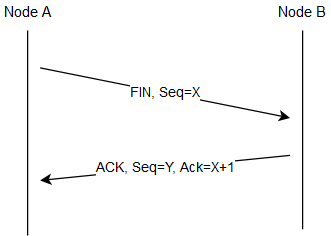
\includegraphics[width=0.70\textwidth]{disconnect_diagram.png}
		    \caption{Diagram procesu ukončenia spojenia}
		    \label{fig:disconnect_diagram}
		\end{figure}


\section{Implementácia}
    Na implementáciu protokolu bola v jayzku Python\footnote{Python v3.10.12 s použitím knižníc \textbf{socket} a \textbf{threading}.} vytvorená komunikačná aplikácia. Tá umožnuje nadviazanie spojenia dvoch uzlov pomocou nášho vlastného protokolu. Pri spustení používateľ zadá IP adresu druhého uzla, port na prijímanie správ a port na odosielanie. Keďže ide o peer-to-peer komunikáciu, po úspešnom spojení si obe strany môžu vymieňať správy až do ukončenia spojenia.\footnote{Vďaka vláknam môžu oba uzly správy aj prijímať, aj posielať}. To môže nastať keď jeden z používateľov napíše "\textbf{/disconnect}", alebo jednoducho vypne aplikáciu. Správanie uzla je zobrazené diagramom v Obr. \ref{fig:workflow}

   \begin{figure}[h]
        \centering
        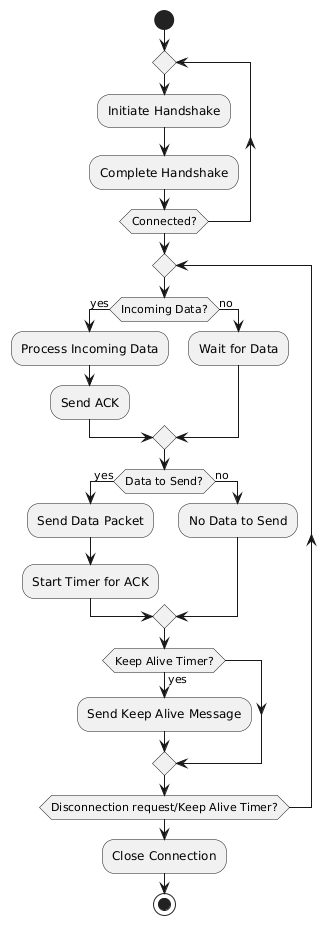
\includegraphics[width=0.5\textwidth]{program_diagram.png}
        \caption{Diagram opisujúci správanie uzla.}
        \label{fig:workflow}
    \end{figure}



    \subsection{Fragmentácia}\label{frag}
    Implementácia podporuje fragmentovaný prenos údajov s maximálnou veľkosťou fragmentu definovanou používateľom. Každý fragment správy nesie informácie o svojej pozícii v kompletnej správe a je očíslovaný rovnakým sekvenčným číslom. Postup prenosu dát pri fragmentácii:

	\begin{enumerate}
		\item Veľká správa sa rozdelí na niekoľko menších fragmentov, pričom každá z nich obsahuje časť pôvodnej správy má rovnaké poradové číslo (sequence number v hlavičke protokolu). Každý fragment má osobitné fragmentové číslo, ktoré označuje jeho poradie medzi zvyšnými fragmentami.\footnote{Maximálna veľkosť fragmentu je okrem používateľského vstupu ohraničená aj maximálnou veľkosťou UDP packetov (${2}^{16}$ bitov).}
		\item Prijímateľ postupne dostane všetky fragmenty, pričom podľa poradového čísla a fragmentového čísla rozpozná, že patria k tej istej správe a v akom poradí ich následne treba poskladať. Pred poskladaním sa každý fragment skontroluje (vypočíta sa checksum pomocou CRC16). Ak je fragment poškodený, odošle sa naspäť hlásenie o chybe (ERR packet) a fragment sa získa od odosielateľa znova.
		\item Nakoniec sa všetky fragmenty zoradia podľa fragmentových čísel a spoja sa do výslednej správy.
	\end{enumerate}


    \subsection{Vytváranie a riešenie chýb}
    Protokol zahŕňa mechanizmy na detekciu a požiadanie o opätovné odoslanie stratených alebo poškodených packetov. Pre ich otestovanie sa v implementácii nachádzajú spôsoby, ako zámerne vytvárať chyby:
	\begin{enumerate}
		\item Náhodná zmena bitov v packete (simulácia poškodenia dát počas prenosu) aby nesedel checksum odosielateľa a checksum prijímateľa.
		\item Zahodenie niektorých packetov.
		\item Duplikovanie niektorých packetov. 
	\end{enumerate}

	Tieto mechanizmy občas naschvál narušia bezchybnú výmenu údajov, s účelom otestovať riešenie chýb pomocou navrhovaného protokolu. Metódy riešenia takýchto problémov sú rozoberané v častiach~\ref{crc}, ~\ref{prenos} a ~\ref{keepalive}. Hlavná myšlienka je, že akékoľvek poškodené alebo stratené packety sa opäť vyžiadajú od odosielateľa, a duplikované packety sú ignorované.


\section{Záver}
	Úspešne sme navrhli a implementovali vlastný protokol na jednoduchý, no spoľahlivý prenos údajov spôsobom \textit{Stop-and-Wait ARQ}. Protokol umožňuje fragmentáciu správ, kontrolu integrity pomocou CRC-16 a zabezpečuje spoľahlivé spojenie vďaka Keep-Alive systému a nadviazaním spojenia cez 3-way handshake. Prenášané packety sú viditeľné prostredníctvom programu Wireshark a sú v nej rozoznateľné polia nášho vlastného protokolu.

\section{Zdroje}
	\begin{itemize}
	    \item \url{https://www.planttext.com/}
	    \item \url{https://app.diagrams.net/}
	    \item \url{https://protocol-designer.app/protocols/9d5267ac-fe04-441b-849c-d9c5c5564e9a}
	    \item \url{https://en.wikipedia.org/wiki/Transmission_Control_Protocol}
	    \item \url{https://en.wikipedia.org/wiki/Cyclic_redundancy_check}
	    \item STEINMETZ, Ralf – WEHRLE, Klaus. 2005. Peer-to-Peer Systems and Applications. Berlin, 2005. 476 s. ISBN 978-3-540-29192-0
	\end{itemize}

\end{document}
